\documentclass{article}

\usepackage{tikz}
\usetikzlibrary{arrows.meta}

\begin{document}
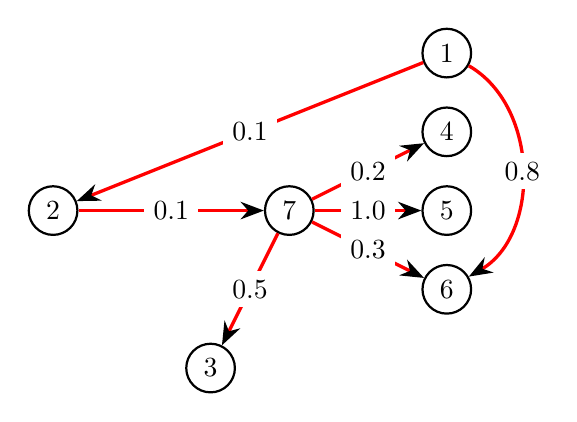
\begin{tikzpicture}

\begin{scope}[every node/.style={circle,thick,draw}]
	\node (1) at (5,4) {1};
	\node (2) at (0,2) {2};
	\node (3) at (2,0) {3};
	\node (4) at (5,3) {4};
	\node (5) at (5,2) {5};
	\node (6) at (5,1) {6};
	\node (7) at (3,2) {7};
\end{scope}

\begin{scope}[>={Stealth[black]},
every node/.style={fill=white},
every edge/.style={draw=red,very thick}]
	\path [->] (1) edge node {$0.1$} (2);
	\path [->] (2) edge node {$0.1$} (7);
	\path [->] (7) edge node {$0.5$} (3);
	\path [->] (7) edge node {$1.0$} (5);
	\path [->] (7) edge node {$0.2$} (4);
	\path [->] (7) edge node {$0.3$} (6);
	\path [->] (1) edge[bend left=60] node {$0.8$} (6);
\end{scope}

\end{tikzpicture}
\end{document}